% Chapter 4, Topic _Linear Algebra_ Jim Hefferon
%  http://joshua.smcvt.edu/linearalgebra
%  2001-Jun-12
\topic{Speed of Calculating Determinants}
For large matrices, finding the determinant by 
using row operations
is typically much faster than using the permutation expansion.
We make this statement 
precise by finding how many operations each method performs.

To compare the speed of two algorithms, we find for each one
how the time taken grows as the size of
its input data set grows.
For instance, if we increase the size of the input by a
factor of ten does the time taken grow by a factor of ten,
or by a factor of a hundred, or by a factor of a thousand?
That is, 
is the time taken proportional to the size of the data set, 
or to the square of that size, or to the cube of that size, etc.? 
An algorithm whose time is proportional to the square is faster than
one that takes time proportional to the cube.

First consider
the permutation expansion formula.\index{determinant!permutation expansion}%
\index{permutation expansion}
\begin{equation*}
   \begin{vmat}
      t_{1,1}  &t_{1,2}  &\ldots  &t_{1,n}  \\
      t_{2,1}  &t_{2,2}  &\ldots  &t_{2,n}  \\
               &\vdots                      \\
      t_{n,1}  &t_{n,2}  &\ldots  &t_{n,n}
   \end{vmat}
   =\!\!\sum_{\text{permutations\ }\phi}\!\!\!\!
     t_{1,\phi(1)}t_{2,\phi(2)}\cdots t_{n,\phi(n)}
                                 \deter{P_{\phi}}   
   % &=
   % \begin{aligned}[t]
   %    &t_{1,\phi_1(1)}\cdot t_{2,\phi_1(2)}\cdots
   %         t_{n,\phi_1(n)}\deter{P_{\phi_1}}       \\  %[.25ex]
   %    &\hbox{}\quad\hbox{}
   %      +t_{1,\phi_2(1)}\cdot t_{2,\phi_2(2)}\cdots
   %         t_{n,\phi_2(n)}\deter{P_{\phi_2}}       \\
   %    &\hbox{}\quad\hbox{}\vdotswithin{+}             \\
   %    &\hbox{}\quad\hbox{}
   %      +t_{1,\phi_k(1)}\cdot t_{2,\phi_k(2)}\cdots
   %         t_{n,\phi_k(n)}\deter{P_{\phi_k}} 
   % \end{aligned}
\end{equation*}
There are
$n!=n\cdot(n-1)\cdots 2\cdot 1$ different \( n \)-permutations so
for a matrix with $n$~rows this sum has $n!$ terms
(and inside each term is $n$-many multiplications). 
The factorial function grows quickly:  
when $n$ is only $10$ the expansion already has  
$10!=3,628,800$ terms. 
Observe that growth proportional to 
the factorial is bigger than growth proportional to the square  $n!>n^2$ 
because multiplying the first
two factors in $n!$ gives $n\cdot(n-1)$, which for large $n$
is approximately $n^2$ and then multiplying in more factors will make the 
factorial even larger.
Similarly, the factorial function grows faster than~$n^3$, 
etc.
So an algorithm that uses the permutation
expansion formula, and thus performs a number of operations
at least as large as the factorial of the number of rows,
would be very slow.

In contrast, the time taken by the row reduction method does not grow so fast.
% Below is a fragment of row-reduction code.
% It is 
% in the computer language \textsc{FORTRAN}, 
% which is widely used for numeric code.
% % (there are no rows below
% % the \lstinline[style=inline]!N!-th 
% % so it is not included in the loop).
% \begin{lstlisting}
% DO 10 ROW=1, N-1
%   PIVINV=1.0/A(ROW,ROW)
%   DO 20 I=ROW+1, N
%     DO 30 J=I, N
%       A(I,J)=A(I,J)-PIVINV*A(ROW,J)
%     30 CONTINUE
%   20 CONTINUE
% 10 CONTINUE
% \end{lstlisting} 
Below is a script for row reduction
in the computer language Python.
(\textit{Note:}
The code here is naive; for example it does not handle the case that 
the \lstinline[style=inline]!m(p_row, p_row)! entry is zero.
Analysis of a finished version that includes all of the tests
and subcases is messier but would gives us roughly the same speed
results.)
\begin{lstlisting}
import random

def random_matrix(num_rows, num_cols):
    m = []
    for col in range(num_cols):
        new_row = []
        for row in range(num_rows):
            new_row.append(random.uniform(0,100))
        m.append(new_row)
    return m

def gauss_method(m):
    """Perform Gauss's Method on m.  This code is for illustration only
    and should not be used in practice.
      m  list of lists of numbers; each included list is a row
    """
    num_rows, num_cols = len(m), len(m[0])
    for p_row in range(num_rows):
        for row in range(p_row+1, num_rows):
            factor = -m[row][p_row] / float(m[p_row][p_row])
            new_row = []
            for col_num in range(num_cols): 
                p_entry, entry = m[p_row][col_num], m[row][col_num]
                new_row.append(entry+factor*p_entry)
            m[row] = new_row
    return m

response = raw_input('number of rows? ')
num_rows = int(response)
m = random_matrix(num_rows, num_rows)
for row in m:
    print row
M = gauss_method(m)
print "-----"
for row in M:
    print row
\end{lstlisting}
Besides a routine to do Gauss's Method, this program also has a routine
to generate a matrix filled with random numbers (the numbers are
between $0$ and~$100$, to make them readable below).
This program prompts a user
for the number of rows, generates a random square matrix of
that size, and does row reduction on it.
\begin{lstlisting}
$ python gauss_method.py
number of rows? 4
[69.48033741746909, 32.393754742132586, 91.35245787350696, 87.04557918402462]
[98.64189032145111, 28.58228108715638, 72.32273998878178, 26.310252241189257]
[85.22896214660841, 39.93894635139987, 4.061683241757219, 70.5925099861901]
[24.06322759315518, 26.699175587284373, 37.398583921673314, 87.42617087562161]
-----
[69.48033741746909, 32.393754742132586, 91.35245787350696, 87.04557918402462]
[0.0, -17.40743803545155, -57.37120602662462, -97.2691774792963]
[0.0, 0.0, -108.66513774392809, -37.31586824349682]
[0.0, 0.0, 0.0, -13.678536859817994]
\end{lstlisting}  %$

Inside of the
\lstinline[style=inline]!gauss_method!
routine, for each row \lstinline[style=inline]!prow!, the routine performs
$\text{\lstinline[style=inline]!factor!}\cdot\rho_{\text{\lstinline[style=inline]!prow!}}+\rho_{\text{\lstinline[style=inline]!row!}}$ 
on the rows below.
For each of these rows below, 
this involves operating on every entry in that row.
That is a triply-nested loop.
So this program has a running time that is something like the  
cube of the number of rows in the matrix.
(\textit{Comment.}
We are glossing over many issues.
For example, we may worry that the time taken by the program
is dominated by the time to store and 
retrieve entries from memory, rather than by the row operations.
However, development of a computation model is outside of
our scope.)

If we add this code at the bottom,
\begin{lstlisting}
def do_matrix(num_rows):
    gauss_method(random_matrix(num_rows, num_rows))

import timeit
for num_rows in [10,20,30,40,50,60,70,80,90,100]:
    s = "do_matrix("+str(num_rows)+")"
    t = timeit.timeit(stmt=s, setup="from __main__ import do_matrix",
                      number=100)
    print "num_rows=", num_rows, " seconds=", t  
\end{lstlisting}
then Python will time the program. 
Here is the output from a timed test run.
\begin{lstlisting}
num_rows= 10  seconds= 0.0162539482117
num_rows= 20  seconds= 0.0808238983154
num_rows= 30  seconds= 0.248152971268
num_rows= 40  seconds= 0.555531978607
num_rows= 50  seconds= 1.05453586578
num_rows= 60  seconds= 1.77881097794
num_rows= 70  seconds= 2.75969099998
num_rows= 80  seconds= 4.10647988319
num_rows= 90  seconds= 5.81125879288
num_rows= 100  seconds= 7.86893582344  
\end{lstlisting}
Graphing that data gives part of the curve of a cubic.
\begin{center}
  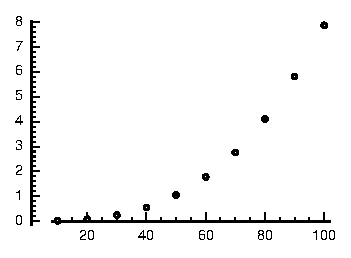
\includegraphics{det/bin/detspeed.pdf}
\end{center}

Finding the fastest algorithm to compute the determinant 
is a topic of current research.
So far, researchers have found algorithms that run in time between the 
square and cube of the number of rows.

The contrast between the times taken by the two determinant computation
methods of permutation expansion and row operations 
makes the point that although in principle they give the same answer, 
in practice we want the one with the best performance.


\begin{exercises}
  % \item[\textit{Most of these presume access to a computer.}]
  \item 
    To get an idea of what happens for typical matrices
    we can use the ability of computer systems to generate random numbers
    (of course, these are only pseudo-random in that they come from
    an algorithm but they 
    pass a number of reasonable statistical tests for randomness).
    \begin{exparts}
      \partsitem Fill a $\nbyn{5}$ array with random numbers say, in the
        range $\clopinterval{0}{1}$).
        See if it is singular.
        Repeat that experiment a few times.
        Are singular matrices frequent or rare in this sense?
      \partsitem Time your computer algebra system at finding the
        determinant of ten $\nbyn{10}$ arrays of random numbers.
        Find the average time per array.
        Repeat the prior item for $\nbyn{20}$ arrays,
        $\nbyn{30}$ arrays, \ldots $\nbyn{100}$ arrays, 
        and compare to the numbers given above.
        (Notice that, when an array is singular, we can sometimes decide that
        quickly,
        for instance if the first row equals the second.
        In the light of your answer to the first part, do you expect that 
        singular systems play a large role in your average?)
      \partsitem Graph the input size versus the average time.
    \end{exparts}
    \begin{answer}
      Your timing will depend in part on the computer algebra system
      that you use, and in part on the power of the computer on which
      you do the calculation.
      But you should get a curve that is similar to the one shown.
%       \begin{exparts}
%         \partsitem Under Octave, \texttt{rank(rand(5))} finds the
%           rank of a $\nbyn{5}$ matrix whose entries are (uniformly
%           distributed) in the interval $[0..1)$.
%           This loop which runs the test $5000$ times
% \begin{lstlisting}
% octave:1> for i=1:5000
% > if rank(rand(5))<5 printf("That's one."); endif
% > endfor
% \end{lstlisting}  
%           produces (after a few seconds) returns the prompt, with no output.

%           The Octave script
% \begin{lstlisting}
% function elapsed_time = detspeed (size)
%   a=rand(size);
%   tic();
%   for i=1:10
%      det(a);
%   endfor
%   elapsed_time=toc();
% endfunction
% \end{lstlisting}  
%           lead to this session (obviously, your times will vary). 
% \begin{lstlisting}
% octave:1> detspeed(5)
% ans = 0.019505
% octave:2> detspeed(15)
% ans = 0.0054691
% octave:3> detspeed(25)
% ans = 0.0097431
% octave:4> detspeed(35)
% ans = 0.017398
% \end{lstlisting}  
%           \partsitem Here is the data (rounded a bit), and the graph.
%             \begin{center}
%               \begin{tabular}{l}
%               \begin{tabular}{r|cccccc}
%                  \textit{matrix rows} 
%                     &$15$ &$25$ &$35$ &$45$ &$55$ &$65$  \\
%                  \hline
%                  \textit{time per ten}
%                     &$0.003\,4$                     
%                     &$0.009\,8$
%                     &$0.067\,5$
%                     &$0.028\,5$ 
%                     &$0.044\,3$
%                     &$0.066\,3$ 
%               \end{tabular}                                       \\
%               \qquad\begin{tabular}{r|ccc}
%                  \textit{matrix rows} 
%                     &$75$ &$85$ &$95$ \\
%                  \hline
%                  \textit{time per ten}
%                     &$0.142\,8$  
%                     &$0.228\,2$ 
%                     &$0.168\,6$              
%               \end{tabular}
%               \end{tabular}
%             \end{center}
%           This data is from an average of twenty runs of the above script,
%           because of the possibility that the randomly chosen matrix
%           happens to take an unusually long or short time.
%           Even so, the timing cannot be relied on too heavily; this is
%           just an experiment.
%           \begin{center}
%             \includegraphics[width=0.4\textwidth]{det/mp/ch4.28}
%           \end{center}
%       \end{exparts}
    \end{answer}
  \item 
    Compute the determinant of each of these by hand using the 
    two methods discussed above.
    \begin{exparts*}
      \partsitem $\begin{vmat}[r]
                    2  &1  \\
                    5  &-3
                  \end{vmat}$
      \partsitem $\begin{vmat}[r]
                    3  &1  &1  \\
                   -1  &0  &5  \\
                   -1  &2  &-2 
                  \end{vmat}$
      \partsitem $\begin{vmat}[r]
                    2  &1  &0  &0  \\
                    1  &3  &2  &0  \\
                    0  &-1 &-2 &1  \\
                    0  &0  &-2 &1
                  \end{vmat}$
    \end{exparts*}
    Count the number of multiplications and divisions used in each case,
    for each of the methods.
    % (Computer multiplications and divisions take 
    %  longer than additions and subtractions, so algorithm 
    %  designers worry about them more.)
     \begin{answer}
       The number of operations depends on exactly how we do the operations.
       \begin{exparts}
         \partsitem The determinant is $-11$.
           To row reduce takes a single row combination 
           with two multiplications
           ($-5/2$ times $2$ plus $5$, and $-5/2$ times $1$ plus $-3$)
           and the product down the diagonal takes one more multiplication.
           The permutation expansion takes two multiplications ($2$ times
           $-3$ and $5$ times $1$).
         \partsitem The determinant is $-39$.
           Counting the operations is routine.
         \partsitem The determinant is $4$.
       \end{exparts}
     \end{answer}
  \item The use by the timing routine of \lstinline[style=inline]!do_matrix!   
    has a bug.
    That routine does two things, generate a random matrix and 
    then do \lstinline[style=inline]!gauss_method! on it, and the 
    timing number returned is for the combination.
    Produce code that times only the 
    \lstinline[style=inline]!gauss_method! routine. 
    \begin{answer}
      You should build the matrix once and then time it being reduced
      many times.
      Note that \lstinline[style=inline]!gauss_method!, as written,
      changes the input matrix, so be careful not to loop using 
      the output of that routine or all the loops but the first will 
      be on an echelon form matrix.
    \end{answer}
  \item 
    What $\nbyn{10}$ array can you invent that takes your computer
    the longest time to reduce?
    The shortest?
    \begin{answer}
      The identity matrix typically does not take long to reduce.
      For matrices that are slow, in Python you can try ones with numbers that
      are quite large.
      (Some computer algebra system also have the ability to generate
      special matrices; try some of those.)
      % One way to get started is to compare these under Octave:
      % \texttt{det(rand(10));}, versus
      % \texttt{det(hilb(10));}, versus
      % \texttt{det(eye(10));}, versus
      % \texttt{det(zeroes(10));}. 
      % You can time them as in \texttt{tic(); det(rand(10)); toc()}.
    \end{answer}
%   \item 
%     Write the rest of the FORTRAN program to do a
%     straightforward implementation of calculating determinants via
%     Gauss's Method.
%     (Don't test for a zero leading entry.)
%     Compare the speed of your code to that used in your computer algebra
%     system.
%     \begin{answer}
%       This is a simple one.
% \begin{lstlisting}
% DO 5 ROW=1, N
%    PIVINV=1.0/A(ROW,ROW)
%    DO 10 I=ROW+1, N
%       DO 20 J=I, N
%          A(I,J)=A(I,J)-PIVINV*A(ROW,J)
%       20 CONTINUE
%    10 CONTINUE
% 5 CONTINUE
% \end{lstlisting}     
%     \end{answer}
  \item Some computer language specifications requires that arrays be
    stored ``by column,'' that is, the entire first column is stored
    contiguously, then the second column, etc.
    Does the code fragment given take advantage of this,
    or can it be rewritten to make it faster, by taking advantage of
    the fact that computer fetches are faster from contiguous locations?
    \begin{answer}
      No, the above code handles the numbers by row.
    \end{answer}
\end{exercises}
\endinput
